\subsubsection{FIFOLevel}
%\subsubsection{Level FIFO}

\index{LevelFIFO|see{FIFOLevel}}
\index{FIFOLevel@\te{FIFOLevel} (package)}
\label{FIFOLevel}

{\bf Package}

%import LevelFIFO :: * ;

\begin{verbatim}
import FIFOLevel :: * ;
\end{verbatim}

{\bf Description}

The BSV \te{FIFOLevel} library provides enhanced FIFO interfaces and modules
which include methods to indicate the level or the current number
of items stored in the FIFO.   Both single clock and dual clock
(separate clocks for the enqueue and dequeue sides)
versions are  included in this package. 

%  The single clock versions are: \te{FIFOLevelIfc} and \te{}.
% The dual clock versions, that is separate clocks for the enqueue and
% dequeue side,  are:
% \te{SyncFIFOLevelIfc} and \te{

{\bf Interfaces and methods}

The \te{FIFOLevelIfc} interface defines methods to compare the current
level to \te{Integer} constants for a single clock.  The
\te{SyncFIFOLevelIfc} defines the same methods for dual clocks; thus
it provides methods for both the source (enqueue) and destination
(dequeue) clock domains.  Instead of methods to compare the levels,
the \te{FIFOCountIfc} and \te{SyncFIFOCountIfc} define methods to
return  counts of the FIFO contents, for single clocks and dual clocks
respectively. 






\begin{tabular}{|p{1.2in}|p{.8in}|p{1.6 in}|p{1.7 in}|}
 \hline
 &  & &   \\
Interface Name   & Parameter name & Parameter Description &
 Requirements of modules implementing the ifc \\
\hline
\hline
\te{FIFOLevelIfc} & \it{element\_type} & type of the elements stored
 in the \te{FIFO} &must be in \te{Bits} class \\
\cline{2-4}
&\it{fifoDepth}&the depth of the \te{FIFO}&must be \te{numeric} type
and >2\\
\hline
\te{FIFOCountIfc} & \it{element\_type} & type of the elements stored
 in the \te{FIFO} &must be in \te{Bits} class \\
\cline{2-4}
&\it{fifoDepth}&the depth of the \te{FIFO}&must be \te{numeric} type
and >2\\
%\cline{2-4}
%&\it{cntSize}&The size of the count&must be \te{numeric} type equal
%to \te{log(fifoDepth + 1)}\\
\hline
\te{SyncFIFOLevelIfc} & \it{element\_type} & type of the elements stored in the \te{FIFO} &must be in \te{Bits} class \\
\cline{2-4}
&\it{fifoDepth}&the depth of the \te{FIFO}&must be \te{numeric} type
and must be a power of 2 and >=2\\
\hline
\te{SyncFIFOCountIfc}&\it{element\_type}& type of the elements stored in the \te{FIFO} &must be in \te{Bits} class \\
\cline{2-4}
&\it{fifoDepth}&the depth of the \te{FIFO}&must be \te{numeric} type
and must be a power of 2 and >=2\\
%\cline{2-4}
%&\it{cntSize}&The size of the counter&must be \te{numeric} type equal
%to \te{log(fifoDepth + 1)}\\
\hline
\end{tabular}

%\begin{itemize}
%\item{\te{FIFOLevelIfc}}
\index{FIFOLevelIfc@\te{FIFOLevelIfc} (interface)}

In addition to common FIFO methods, the \te{FIFOLevelIfc}
interface defines methods to compare the current level to 
\te{Integer} constants.  See Section \ref{sec-FIFO} for details on
\te{enq}, \te{deq}, \te{first}, \te{clear}, \te{notFull}, and \te{notEmpty}.
Note that \te{FIFOLevelIfc} interface has a type parameter for the
\te{fifoDepth}.  This numeric type parameter is needed, since the width
of the counter is dependent on the FIFO depth.
The \te{fifoDepth} parameter must be $> 2$.  



\begin{center}
\begin{tabular}{|p{.9in}|p{.4in}|p{1.8 in}|p{.4in}|p{1.3 in}|}
\hline
\multicolumn{5}{|c|}{FIFOLevelIfc}\\
\hline
\multicolumn{3}{|c|}{Method}&\multicolumn{2}{|c|}{Argument}\\
\hline
Name & Type & Description& Name &\multicolumn{1}{|c|}{Description} \\
\hline
\hline 
\te{isLessThan}&Bool&Returns \te{True} if the depth of the
\te{FIFO} is less than the \te{Integer} constant, \te{c1}.&c1&an \te{Integer}
compile-time constant\\
\hline
\te{isGreaterThan}&Bool&Returns  \te{True}  if the depth of the
\te{FIFO} is greater than the \te{Integer} constant, \te{c1}.&c1&an
\te{Integer} compile-time constant\\ 
\hline
\end{tabular}
\end{center}

\begin{libverbatim}
interface FIFOLevelIfc#( type element_type, numeric type fifoDepth ) ;
   method Action enq( element_type x1 );
   method Action deq();
   method element_type first();
   method Action clear();

   method Bool notFull ;
   method Bool notEmpty ;

   method Bool isLessThan   ( Integer c1 ) ;
   method Bool isGreaterThan( Integer c1 ) ;
endinterface 
\end{libverbatim}

\index{FIFOCountIfc@\te{FIFOCountIfc} (interface)}

In addition to common FIFO methods, the \te{FIFOCountIfc}
interface defines a method  to return the  current number of elements as an 
bit-vector.  See Section \ref{sec-FIFO} for details on
\te{enq}, \te{deq}, \te{first}, \te{clear}, \te{notFull}, and \te{notEmpty}.
Note that the \te{FIFOCountIfc} interface has a type parameter for the
\te{fifoDepth}.  This numeric type parameter is needed, since the width
of the counter is dependent on the FIFO depth.  The \te{fifoDepth}
parameter  must be $> 2$.  

\begin{center}
\begin{tabular}{|p{.5 in}|p{2.3 in}|p{2.5 in}|}
\hline
\multicolumn{3}{|c|}{FIFOCountIfc}\\
\hline
\multicolumn{3}{|c|}{Method}\\
\hline
Name & Type & Description\\
\hline
\hline
\te{count}&UInt\#(TLog\#(TAdd\#(fifoDepth,1)))&Returns the number of items in the
\te{FIFO}.\\
\hline
\end{tabular}
\end{center}


\begin{libverbatim}
interface FIFOCountIfc#( type element_type, numeric type fifoDepth) ;
   method Action enq ( element_type sendData ) ;
   method Action deq () ;
   method element_type first () ;

   method Bool notFull ;
   method Bool notEmpty ;
   
   method UInt#(TLog#(TAdd#(fifoDepth,1))) count;

   method Action clear;
endinterface 
\end{libverbatim}

%\item{\te{SyncFIFOLevelIfc}}

The interfaces \te{SyncFIFOLevelIfc} and \te{SyncFIFOCountIfc} are dual
clock versions of the \te{FIFOLevelIfc} and \te{FIFOCountIfc}.
Methods are provided for both source and destination clock domains.
The following
table describes the dual clock  \te{notFull} and
\te{notEmpty} methods, as well as the dual clock \te{clear} methods, which are common to both interfaces.  
Note that the
\te{SyncFIFOLevelIfc} and \te{SyncFIFOCountIfc} interfaces each have a type
parameter  for \te{fifoDepth}.  This numeric type parameter is needed, since the width
of the counter is dependent on the FIFO depth.  The \te{fifoDepth}
parameter must be a power of 2 and $>=2$.  

\begin{center}
\begin{tabular}{|p{1.1in}|p{.4in}|p{3.5 in}|}
%\begin{tabular}{|p{1.1in}|p{.4in}|p{1.6 in}|p{.4in}|p{1.3 in}|}
\hline
\multicolumn{3}{|c|}{Common Dual Clock Methods}\\
\hline
% \multicolumn{3}{|c|}{Method}\\
% \hline
Name & Type & Description\\
\hline
\hline
\te{sNotFull} & Bool & Returns \te{True} if the \te{FIFO} appears as not
full from the source side clock.  \\
\hline
%\end{tabular}
%\end{center}
%\begin{center}
%\begin{tabular}{|p{1.1in}|p{.4in}|p{3.3 in}|}
%\hline
\te{sNotEmpty} & Bool &Returns \te{True} if the \te{FIFO} appears as
not empty from the source side clock.\\
\hline
%\end{tabular}
%\end{center}
%\begin{center}
%\begin{tabular}{|p{1.1in}|p{.4in}|p{3.3 in}|}
%\hline
\te{dNotFull} & Bool & Returns \te{True} if  the \te{FIFO} appears as
not full from the destination side clock.\\
\hline
%\end{tabular}
%\end{center}
%\begin{center}
%\begin{tabular}{|p{1.1in}|p{.4in}|p{3.3 in}|}
%\hline
\te{dNotEmpty} & Bool &Returns \te{True} if the \te{FIFO} appears as
not empty from the destination side clock.\\
\hline
\te{sClear}&Action&Clears the FIFO from the source side.\\
\hline
\te{dClear}&Action&Clears the FIFO from the destination side.\\
\hline
\end{tabular}
\end{center}


\index{SyncFIFOLevelIfc@\te{SyncFIFOLevelIfc} (interface)}
In addition to common FIFO methods (Section \ref{sec-FIFO}) and the
common dual clock methods above, the \te{SyncFIFOLevelIfc}
interface defines methods to compare the current level to 
\te{Integer} constants.  Methods are provided for both the source
(enqueue side) and destination (dequeue side) clock domains.%  Note that
% \te{SyncFIFOLevelIfc} interface has a type parameter for 
% \te{fifoDepth}.  This numeric type parameter is needed, since the width
% of the counter is dependent on the FIFO depth.  The \te{fifoDepth}
% parameter must be a power of 2 and >=2.  A \te{fifoDepth} of 1 will
% generate a  compile time ``out of range'' error
 
   
\begin{center}
\begin{tabular}{|p{1 in}|p{.4 in}|p{2 in}|p{.4 in}|p{1.3 in}|}
\hline
\multicolumn{5}{|c|}{SyncFIFOLevelIfc Methods}\\
\hline
\multicolumn{3}{|c|}{Method}&\multicolumn{2}{|c|}{Argument}\\
\hline
Name & Type & Description& Name &\multicolumn{1}{|c|}{Description} \\
\hline
\hline
\te{sIsLessThan}&Bool&Returns \te{True} if the depth of the
\te{FIFO}, as appears on the source side clock, is less than the
\te{Integer} constant, \te{c1}.&c1&an \te{Integer}
compile-time constant\\
\hline
% \end{tabular}
% \end{center}
% \begin{center}
% \begin{tabular}{|p{1.1in}|p{.4in}|p{1.6 in}|p{.4in}|p{1.3 in}|}
% \hline
\te{sIsGreaterThan}&Bool&Returns \te{True} if the depth of the
\te{FIFO}, as it appears on the source side clock, is greater than the
\te{Integer} constant, \te{c1}.&c1&an \te{Integer} compile-time constant.\\
\hline
% \end{tabular}
% \end{center}
% \begin{center}
% \begin{tabular}{|p{1.1in}|p{.4in}|p{1.6 in}|p{.4in}|p{1.3 in}|}
% \hline
\te{dIsLessThan}&Bool&Returns \te{True} if the depth of the
\te{FIFO}, as it appears on the destination side clock, is less than the
\te{Integer} constant, \te{c1}.&c1&an \te{Integer}
compile-time constant\\
\hline
% \end{tabular}
% \end{center}
% \begin{center}
% \begin{tabular}{|p{1.1in}|p{.4in}|p{1.6 in}|p{.4in}|p{1.3 in}|}
% \hline
\te{dIsGreaterThan}&Bool&Returns \te{True} if the depth of the
\te{FIFO}, as appears on the destination side clock, is greater than the
\te{Integer} constant, \te{c1}.&c1&an \te{Integer} compile-time constant.\\
\hline
\end{tabular}
\end{center}

\begin{libverbatim}
interface SyncFIFOLevelIfc#( type element_type, numeric type fifoDepth ) ;
   method Action enq ( element_type sendData ) ;
   method Action deq () ;
   method element_type first () ;

   method Bool sNotFull ;
   method Bool sNotEmpty ;
   method Bool dNotFull ;
   method Bool dNotEmpty ;

   method Bool sIsLessThan   ( Integer c1 ) ;
   method Bool sIsGreaterThan( Integer c1 ) ;
   method Bool dIsLessThan   ( Integer c1 ) ;
   method Bool dIsGreaterThan( Integer c1 ) ;

   method Action sClear;
   method Action dClear;
endinterface 
\end{libverbatim}

\index{SyncFIFOCountIfc@\te{SyncFIFOCountIfc} (interface)}
In addition to common FIFO methods (Section \ref{sec-FIFO}) and the
common dual clock methods above, the \te{SyncFIFOCountIfc} 
interface defines methods to return the  current number of elements.
Methods are provided for both the source
(enqueue side) and destination (dequeue side) clock domains. 
 
   
\begin{center}
\begin{tabular}{|p{.5 in}|p{2.3 in}|p{2.5 in}|}
\hline
\multicolumn{3}{|c|}{SyncFIFOCountIfc}\\
\hline
\multicolumn{3}{|c|}{Method}\\
\hline
Name & Type & Description\\
\hline
\hline
% \te{sNotFull} & Bool & Returns \te{True} if the \te{FIFO} appears as not
% full from the source side clock.  \\
% \hline
% \te{sNotEmpty} & Bool &Returns \te{True} if the \te{FIFO} appears as
% not empty from the source side clock.\\
% \hline
% \te{dNotFull} & Bool & Returns \te{True} if  the \te{FIFO} appears as
% not full from the destination side clock.\\
% \hline
% \te{dNotEmpty} & Bool &Returns \te{True} if the \te{FIFO} appears as
% not empty from the destination side clock.\\
% \hline
% \end{tabular}
% \end{center}
% \begin{center}
%\begin{tabular}{|p{1.1in}|p{.4in}|p{1.6 in}|p{.4in}|p{1.3 in}|}
%\hline
\te{sCount}&UInt\#(TLog\#(TAdd\#(fifoDepth,1)))&Returns the number of items in the
\te{FIFO} from the source side.\\
\hline
\te{dCount}&UInt\#(TLog\#(TAdd\#(fifoDepth,1)))&Returns the number of items in the
\te{FIFO} from the destination side.\\
\hline
\end{tabular}
\end{center}

\begin{verbatim}
interface SyncFIFOCountIfc#( type element_type, numeric type fifoDepth) ;
   method Action enq ( element_type sendData ) ;
   method Action deq () ;
   method element_type first () ;

   method Bool sNotFull ;
   method Bool sNotEmpty ;
   method Bool dNotFull ;
   method Bool dNotEmpty ;
   
   method UInt#(TLog#(TAdd#(fifoDepth,1))) sCount;
   method UInt#(TLog#(TAdd#(fifoDepth,1))) dCount;
      
   method Action sClear;
   method Action dClear;
endinterface 
\end{verbatim}

The \te{FIFOLevelIFC}, \te{SyncFIFOLevelIfc}, \te{FIFOCountIfc}, and \te{SyncFIFOCountIfc} interfaces belong to the \te{ToGet} and
\te{ToPut} typeclasses.  You can use the \te{toGet} and \te{toPut}
functions to convert these interfaces to \te{Get}
and \te{Put} interfaces (Section \ref{sec-GetPut}). 


   
%\end{itemize}

{\bf Modules}
   
\index{mkFIFOLevel@\te{mkFIFOLevel} (module)}
\index[function]{FIFOLevel!mkFIFOLevel}
%\begin{itemize}
%\item{\te{mkFIFOLevel}}

The module  \te{mkFIFOLevel} provides the
\te{FIFOLevelIfc} interface.  Note that the implementation allows any
number of \te{isLessThan} and \te{isGreaterThan} method calls.  Each
call with a unique argument adds an additional comparator to
the design.

There is also available a guarded (G) version of 
\te{FIFOLevel} which takes three  Boolean
parameters; \te{ugenq}, \te{ugdeq}, and \te{ugcount}.  Setting any of
the  parameters to 
\te{TRUE} indicates the method (\te{enq} for \te{ugenq}, \te{deq} for
\te{ugdeq}, and \te{isLessThan}, \te{isGreaterThan} for
\te{ugcount}) is  unguarded.    If all three are
\te{FALSE} the behavior is the same as a regular \te{FIFOLevel}.  


\begin{center}
\begin{tabular}{|p{.9 in}|p{4.4 in}|}
 \hline
&         \\
Module Name  &  BSV Module Declaration  \\
\hline
\hline 
\te{mkFIFOLevel} 
& \begin{libverbatim}
module mkFIFOLevel (
          FIFOLevelIfc#(element_type, fifoDepth) )
   provisos( Bits#(element_type, width_element )
             Log#(TAdd#(fifoDepth,1),cntSize) ) ;
\end{libverbatim} 
\\
\cline{2-2}
&Comment: \te{width\_element} may be 0\\
\hline
\end{tabular}
\end{center}

\index{mkGFIFOLevel@\te{mkGFIFOLevel} (module)}
\index[function]{FIFOLevel!mkGFIFOLevel}

\begin{center}
\begin{tabular}{|p{.9 in}|p{4.4 in}|}
 \hline
&         \\
Module Name  &  BSV Module Declaration  \\
\hline
\hline 
\te{mkGFIFOLevel} 
& \begin{libverbatim}
module mkGFIFOLevel#(Bool ugenq, Bool ugdeq, Bool ugcount)
           ( FIFOLevelIfc#(element_type, fifoDepth) )
   provisos( Bits#(element_type, width_element ),
            Log#(TAdd#(fifoDepth,1),cntSize)); 
\end{libverbatim} 
\\
\cline{2-2}
&Comment: \te{width\_element} may be 0\\
\hline
\end{tabular}
\end{center}


\index{mkFIFOCount@\te{mkFIFOCount} (module)}
\index[function]{FIFOLevel!mkFIFOCount}
\index{mkGFIFOCount@\te{mkGFIFOCount} (module)}
\index[function]{FIFOLevel!mkGFIFOCount}


The  module \te{mkFIFOCount} provides the interface  \te{FIFOCountIfc}.
There is also available a guarded (G) version of 
\te{FIFOCount} which takes three  Boolean
parameters; \te{ugenq}, \te{ugdeq}, and \te{ugcount}.  Setting any of
the  parameters to 
\te{TRUE} indicates the method (\te{enq} for \te{ugenq}, \te{deq} for
\te{ugdeq}, and \te{count} for
\te{ugcount}) is  unguarded.    If all three are
\te{FALSE} the behavior is the same as a regular \te{FIFOCount}.  

\begin{center}
\begin{tabular}{|p{.9 in}|p{4.4 in}|}
 \hline
&         \\
Module Name  &  BSV Module Declaration  \\
\hline
\hline 
\te{mkFIFOCount} 
& \begin{libverbatim}
module mkFIFOCount( 
          FIFOCountIfc#(element_type, fifoDepth) ifc ) 
   provisos (Bits#(element_type, width_element));
\end{libverbatim} 
\\
\cline{2-2}
&Comment: \te{width\_element} may be 0\\
\hline
\end{tabular}
\end{center}


\begin{center}
\begin{tabular}{|p{.9 in}|p{4.4 in}|}
 \hline
&         \\
Module Name  &  BSV Module Declaration  \\
\hline
\hline 
\te{mkGFIFOCount} 
& \begin{libverbatim}
module mkGFIFOCount#(Bool ugenq, Bool ugdeq, Bool ugcount)
         ( FIFOCountIfc#(element_type, fifoDepth) ifc ) 
   provisos (Bits#(element_type, width_element));
\end{libverbatim} 
\\
\cline{2-2}
&Comment: \te{width\_element} may be 0\\
\hline
\end{tabular}
\end{center}


\index[function]{FIFOLevel!mkSyncFIFOLevel}
\index{mkSyncFIFOLevel@\te{mkSyncFIFOLevel} (module)}
%\item{\te{mkSyncFIFOLevel}}

The modules \te{mkSyncFIFOLevel} and \te{mkSyncFIFOCount} are dual
clock FIFOs, where enqueue and 
dequeue methods are in separate clocks domains, \te{sClkIn} and
\te{dClkIn} respectively.  Because of the synchronization latency, the
flag indicators will not necessarily be identical between the source
and the destination clocks.  Note
however, that the \te{sNotFull} and \te{dNotEmpty} flags always give proper
(pessimistic) indications for the safe use of \te{enq} and \te{deq} methods;
these are automatically included as implicit condition in the \te{enq}
and  \te{deq} (and \te{first}) methods. 

The module \te{mkSyncFIFOLevel} provides the \te{SyncFIFOLevelIfc} interface.

\begin{center}
\begin{tabular}{|p{1.1 in}|p{4.2 in}|}
 \hline
&         \\
Module Name  &  BSV Module Declaration  \\
\hline
\hline 
\te{mkSyncFIFOLevel} 
& \begin{libverbatim}
module mkSyncFIFOLevel( 
          Clock sClkIn, Reset sRstIn,
          Clock dClkIn,
          SyncFIFOLevelIfc#(element_type, fifoDepth) ifc ) 
   provisos( Bits#(element_type, width_element), 
             Log#(TAdd#(fifoDepth,1),cntSize));   
\end{libverbatim} 
\\
\cline{2-2}
&Comment: \te{width\_element} may be 0\\
\hline
\end{tabular}
\end{center}


\index[function]{FIFOLevel!mkSyncFIFOCount}
\index{mkSyncFIFOCount@\te{mkSyncFIFOCount} (module)}

\begin{figure}[ht]
\begin{center}
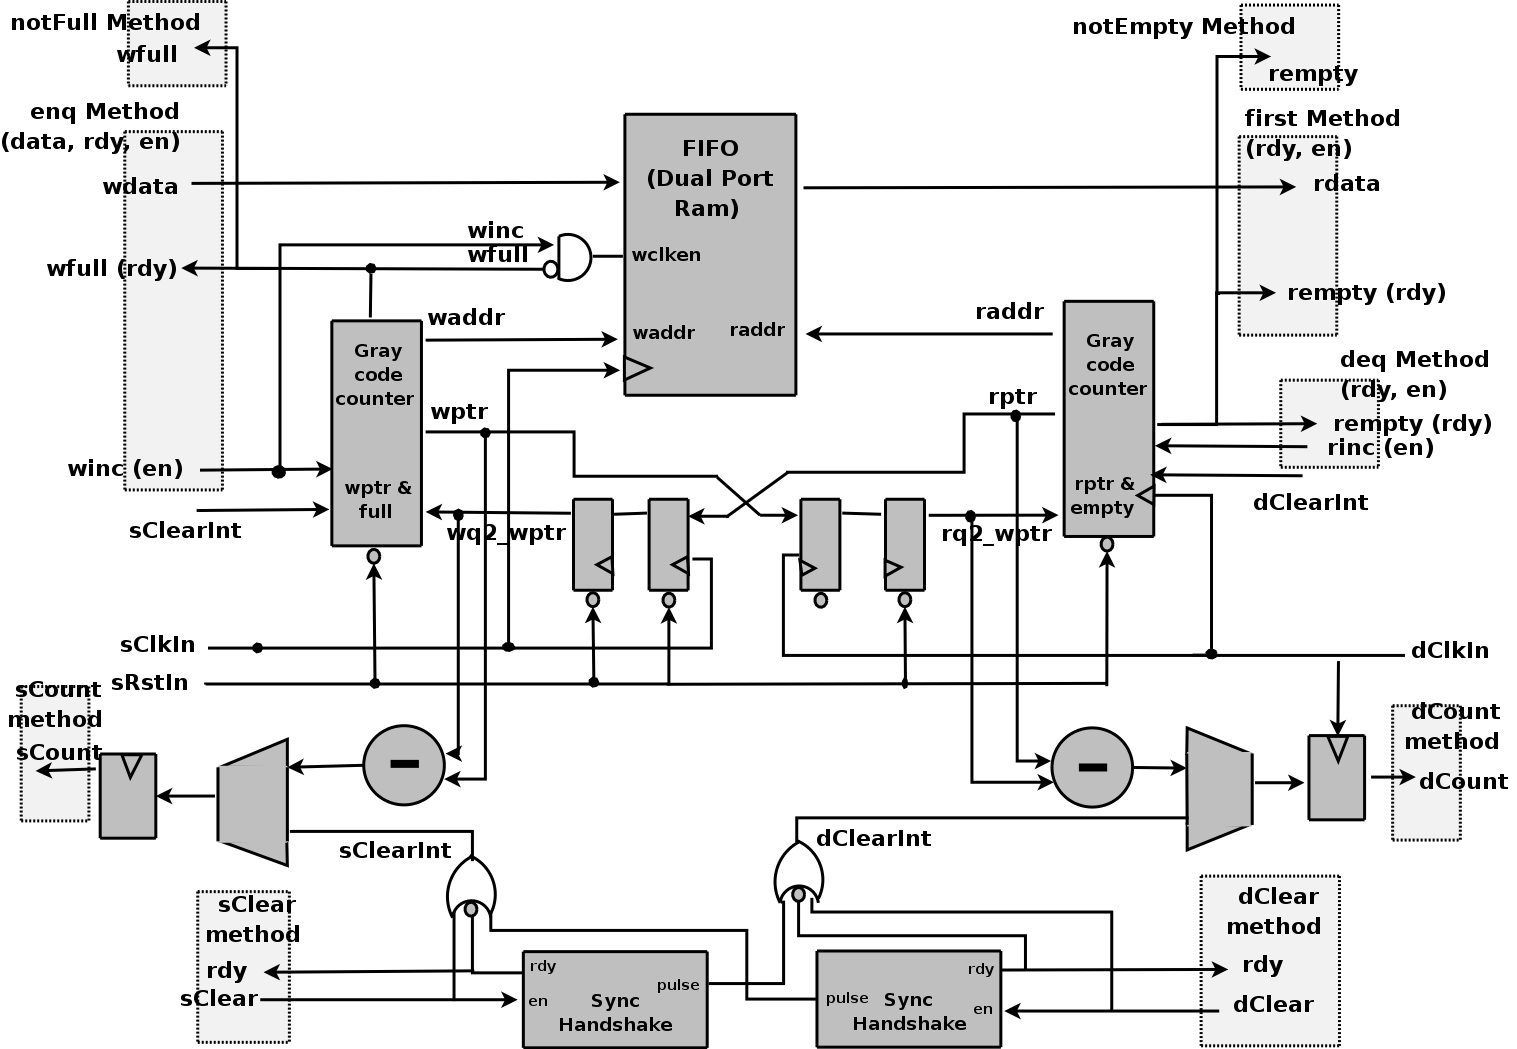
\includegraphics[width  = 5.5 in]{LibFig/syncfifocount}
\caption{SyncFIFOCount}
\label{syncfifocount}
\end{center}
\end{figure}


The module \te{mkSyncFIFOCount}, as shown in Figure
\ref{syncfifocount}  provides the \te{SyncFIFOCountIfc}
interface.  Because of the synchronization latency, the
count reports may  be different between the source
and the destination clocks.  Note
however, that the \te{sCount} and \te{dCount} reports give pessimistic
values with the appropriate side.  That is, the count \te{sCount} (on
the enqueue clock) will report the exact count of items in the FIFO or
a larger count.  The larger number is due to the 
synchronization delay in observing the dequeue action.  Likewise, the
\te{dCount} (on the dequeue clock) returns the exact count or a smaller
count.  The maximum disparity between \te{sCount} and \te{dCount}
depends on the difference in clock periods between the source and
destination clocks.

The module provides \te{sClear}  and \te{dClear}
methods, both of which cause the contents of the FIFO to be removed.
Since the clears must be synchronized and acknowledged from one domain
to the other, there is a non-trivial delay before the FIFO recovers
from the clear and can accept additional enqueues or dequeues
(depending on which side is cleared).  The calling of
either method immediately  disables other activity in the calling
domain. That is, calling \te{sClear} in cycle \te{n} causes the
enqueue to become unready in the next cycle, \te{n+1}.  Likewise, calling
\te{dClear} in cycle \te{n} causes the dequeue to become unready in
the next cycle, \te{n+1}.

%  That
% is, calling \te{sClear} in cycle \te{n} causes the method
% \te{sFull\_N} to return False (the Verilog port \te{sFULL\_N} is
% deasserted) and  \te{sCount} to return  $0$ in cycle \te{n+1}.
%  Further enqueues are disabled.  Likewise, calling \te{dClear} in
% cycle \te{n} causes the method \te{dEmpty\_N} to be asserted and \te{dCount} to
% be $0$ in cycle \te{n+1}.

After the \te{sClear} method is called, the FIFO appears empty on the
dequeue side after three \te{dClock} edges.  Three \te{sClock} edges later,
the FIFO returns to a state where new items can be enqueued.  The
latency is due to the full handshaking synchronization required to
send the clear signal to \te{dClock} and receive the acknowledgement back.

For the \te{dClear} method call, the enqueue side is cleared in three \te{sClkIn} edges and items can be enqueued at the fourth edge.  All
items enqueued at or before the clear are removed from the FIFO.

Note that there is a ready signal associated with both  \te{sClear}
and \te{dClear}
methods to ensure that the clear is properly sent between the clock
domains.  Also,  \te{sRstIn} must be synchronized with the \te{sClkIn}.

\begin{center}
\begin{tabular}{|p{1.1 in}|p{4.2 in}|}
 \hline
&         \\
Module Name  &  BSV Module Declaration  \\
\hline
\hline 
\te{mkSyncFIFOCount} 
& \begin{libverbatim}
module mkSyncFIFOCount( 
          Clock sClkIn, Reset sRstIn,
          Clock dClkIn,
          SyncFIFOCountIfc#(element_type, fifoDepth) ifc ) 
   provisos( Bits#(element_type, width_element));  
\end{libverbatim} 
\\
\cline{2-2}
&Comment: \te{width\_element} may be 0\\
\hline
\end{tabular}
\end{center}

%\end{itemize}
      
{\bf Example}
   
The following example shows the use of \te{SyncFIFOLevel} as a way
to collect data into a FIFO, and then send it out in a burst mode.  The
portion of the design shown, waits until the FIFO is almost
full, and then sets a register, {\tt burstOut} which indicates
that the FIFO should dequeue. When the FIFO is almost empty, the
flag is cleared, and FIFO fills again.

\begin{libverbatim}
   . . .
   // Define a fifo of Int(#23) with 128 entries
   SyncFIFOLevelIfc#(Int#(23),128) fifo <- mkSyncFIFOLevel(sclk, rst, dclk ) ;
  
   // Define some constants 
   let sFifoAlmostFull = fifo.sIsGreaterThan( 120 ) ;
   let dFifoAlmostFull = fifo.dIsGreaterThan( 120 ) ;
   let dFifoAlmostEmpty = fifo.dIsLessThan( 12 ) ;
  
   // a register to indicate a burst mode
   Reg#(Bool)  burstOut <- mkReg( False, clocked_by (dclk)) ;
  
   . . .
   // Set and clear the burst mode depending on fifo status
   rule timeToDeque( dFifoAlmostFull && ! burstOut ) ;
      burstOut <= True ;
   endrule
  
  
   rule moveData ( burstOut ) ;
      let dataToSend = fifo.first ;
      fifo.deq ;
      ...
      burstOut <= !dFifoAlmostEmpty;

   endrule
\end{libverbatim}


{\bf Scheduling Annotations}

Scheduling constraints describe how methods interact within the
schedule.
The annotations for \te{mkFIFOLevel} and \te{mkSyncFIFOLevel} are the
same, except that 
methods in different domains (source and destination) are always
conflict free.


\begin{center}
\begin{tabular}{|c|c|c|c|c|c|c|c|c|}
%begin{tabular}{|p{.75 in}|c|c|c|c|}
\hline
\multicolumn{9}{|c|}{Scheduling Annotations}\\
\multicolumn{9}{|c|}{\te{mkFIFOLevel}, \te{mkSyncFIFOLevel}}\\
\hline
&enq&first&deq&clear&notFull&notEmpty&isLessThan&isGreaterThan\\
\hline
\hline
enq&C &CF&CF&SB&SA&SA&SA&SA\\
\hline
first&CF&CF&SB&SB&CF&CF&CF&CF\\
\hline
deq&CF &SA&C&SB&SA&SA&SA&SA\\
\hline
clear&SA&SA&SA&SBR&SA&SA&SA&SA\\
\hline
notFull&SB&CF&SB&SB&CF&CF&CF&CF\\
\hline
notEmpty&SB&CF&SB&SB&CF&CF&CF&CF\\
\hline
isLessThan&SB&CF&SB&SB&CF&CF&CF&CF\\
\hline
isGreaterThan&SB&CF&SB&SB&CF&CF&CF&CF\\
\hline
\hline
\end{tabular}
\end{center}

The annotations for \te{mkFIFOCount} and \te{mkSyncFIFOCount} are the
same, except that 
methods in different domains (source and destination) are always
conflict free.


\begin{center}
\begin{tabular}{|c|c|c|c|c|c|c|c|}
\hline
\multicolumn{8}{|c|}{Scheduling Annotations}\\
\multicolumn{8}{|c|}{\te{mkFIFOCount}, \te{mkSyncFIFOCount}}\\
\hline
&enq&first&deq&clear&notFull&notEmpty&count\\
\hline
\hline
enq&C&CF&CF&SB&SA&SA&SA\\
\hline
first&CF &CF&SB&SB&CF&CF&CF\\
\hline
deq&CF &SA&C&SB&SA&SA&SA\\
\hline
clear&SA&SA&SA&SBR&SA&SA&SA\\
\hline
notFull&SB&CF&SB&SB&CF&CF&CF\\
\hline
notEmpty&SB&CF&SB&SB&CF&CF&CF\\
\hline
count&SB&CF&SB&SB&CF&CF&CF\\
\hline
\hline
\end{tabular}
\end{center}






{\bf Verilog Modules}

The modules described in this section  correspond to the following {\V}
modules, which are found in the BSC {\V} library,
\te{\$BLUESPECDIR/Verilog/}.  

\begin{center}
\begin{tabular} {|p{2 in}|p{1.5 in}p{1.5 in}|}
\hline
&& \\
BSV Module Name &\multicolumn{2}{|c|}{ Verilog Module Names}  \\
&& \\
\hline
\hline
\begin{libverbatim}mkFIFOLevel
mkFIFOCount
\end{libverbatim}
& \te{SizedFIFO.v} & \te{SizedFIFO0.v} \\
\hline
\begin{libverbatim}mkSyncFIFOLevel
mkSyncFIFOCount
\end{libverbatim}
&\te{SyncFIFOLevel.v}&\\
\hline
\end{tabular}
\end{center}

